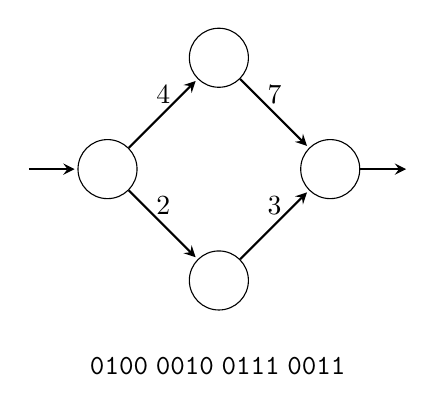
\begin{tikzpicture}
  [->, >=stealth, shorten >=1pt,auto,node distance=2cm,
    align=center,
    neuron/.style={
      circle, draw, minimum size=0.75cm
    },
  ]
  \node[neuron] (i1) {};
  \node[neuron] (h1) [above right of=i1]  {};
  \node[neuron] (h2) [below right of=i1] {};
  \node[neuron] (o1) [below right of=h1] {};

  % Input and output arrows 
  \draw[->, thick] ++(-1, 0) -- (i1);
  \draw[->, thick] (o1) -- ++(1, 0);

  % Edges between nodes
  \path[->, thick]
  (i1) edge node [above] {4} (h1)
       edge node [above] {2} (h2)
  (h1) edge node [above] {7} (o1)
  (h2) edge node [above] {3} (o1);

  \node[yshift=-2.5cm, xshift=1.4cm] () {$\mathtt{0100}\; \mathtt{0010}\; \mathtt{0111}\; \mathtt{0011}$};
\end{tikzpicture}
